\documentclass[12pt]{article}
\usepackage[top=1in, bottom=1in, left=1in, right=1in]{geometry}
\usepackage{paralist}
\usepackage{graphicx}
\usepackage{titlesec}  
\usepackage{amssymb}
\usepackage{amsmath} 
\usepackage{xcolor}

\begin{document}
\title{STAT 498 B Patterns in Randomness}
\author{Nan Tang 1662478}
\date{\today}
\maketitle

\section*{Q1}
\begin{verbatim}
#Simulate 100 sets with x, y variable, each of them has a sample size of 20.
#Plot samples with p-values < 0.05, and calculate the rate of statistically significant samples.
simulations <- 100
signifSum <- 0
par(mfrow = c(3, 3)) #set up a 3 * 3 grid.

for(i in 1 : simulations) {
  y <- rnorm(n = 20, mean = 50, sd = 3)
  x <- rnorm(n = 20, mean = 10, sd = 1)
  reg <- lm(y~x)
  pVal <- summary(reg)$coefficients[2,4]
  if (pVal < 0.05) {
    plot(x, y, pch = 16, col = "skyblue")
    abline(reg, lty = 1, col = "skyblue4")
    signifSum <- signifSum + 1
  }
}
signifRate <- signifSum / simulations
signifRate
##Result is 0.05
\end{verbatim}

\noindent \textcolor{darkgray}{Under the significance level of 0.05, we have 5 samples among 100 simulations that are statistically significant. Four of them displayed a positive relationship between x and y, while one of them showed a negative relationship.}

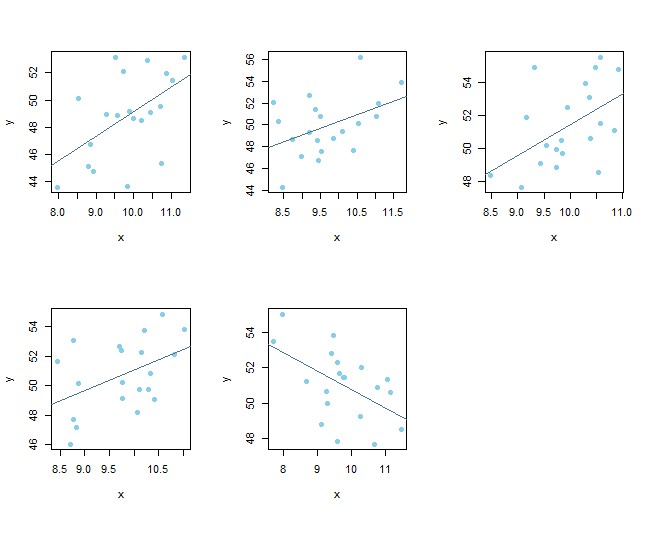
\includegraphics[width = 6 in]{RandPlot1-pv005.jpg}

\begin{verbatim}
par(mfrow = c(3, 3))
signifSum <- 0

for(i in 1 : simulations) {
  y <- rnorm(n = 20, mean = 50, sd = 3)
  x <- rnorm(n = 20, mean = 10, sd = 1)
  reg <- lm(y~x)
  pVal <- summary(reg)$coefficients[2,4]
  if (pVal < 0.1) {
    plot(x, y, pch = 16, col = "skyblue")
    abline(reg, lty = 1, col = "skyblue4")
    signifSum <- signifSum + 1
  }
}
signifRate <- signifSum / simulations
signifRate
##Result is 0.09
\end{verbatim}

\noindent \textcolor{darkgray}{Under the significance level of 0.1, we have 9 samples among 100 are significant. Seven of them displayed a positive relation, while two of them showed negative relation. As my expectation, the ratio of x, y being positive or negatively related should be 50$\%$ each.}

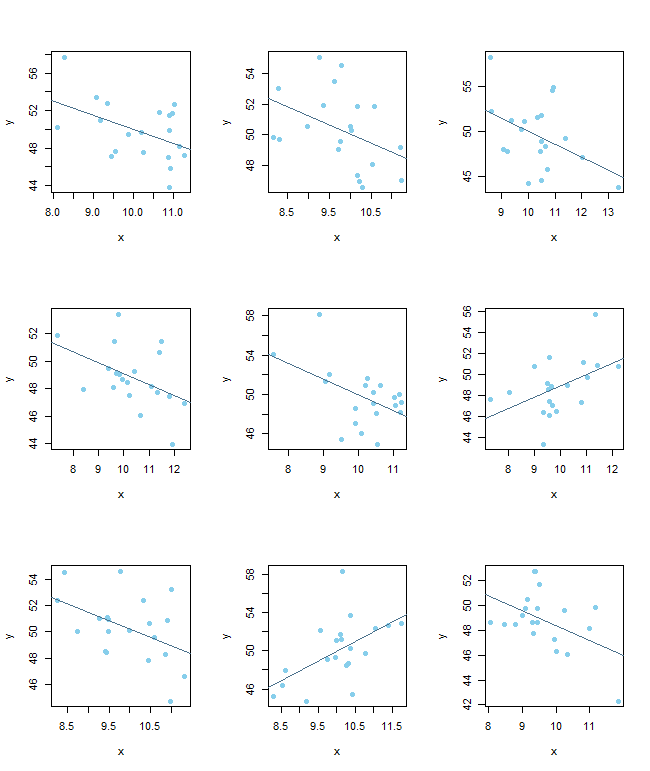
\includegraphics[width = 6 in]{RandPlot2-pv01.png}


\section*{Q2}
\begin{verbatim}
#Simulate 1000 sets with x, y, which both come from independent normal distributions.
#Remove largest residual from each sample.
#Calculate the rate of statistically significant samples after being removed of largest residual.
signifSum <- 0
simulations <- 1000

for (i in 1 : simulations) {
  y <- rnorm(n = 20, mean = 50, sd = 3)
  x <- rnorm(n = 20, mean = 10, sd = 1)
  reg <- lm(y~x)
  largestRes <- which.max(abs(resid(reg)))
  revised_x <- x[-largestRes]
  revised_y <- y[-largestRes]
  revisedReg <- lm(revised_y~revised_x)
  pVal <- summary(revisedReg)$coefficients[2,4]
  if (pVal < 0.05) {
    signifSum <- signifSum + 1
  }
}
signifRate <- signifSum / simulations
signifRate
##Result is 0.096
\end{verbatim}

\noindent \textcolor{darkgray}{After deleting the largest residual in each random sample, we found 9.6$\%$ of simulations are significant (alpha = 0.05). We found that the proportion of significant samples after deletion of largest residual is larger than that before.}

\begin{verbatim}
signifSum <- 0
for (i in 1 : simulations) {
  y <- rnorm(n = 20, mean = 50, sd = 3)
  x <- rnorm(n = 20, mean = 10, sd = 1)
  reg <- lm(y~x)
  largestRes <- which.max(abs(resid(reg)))
  revised_x <- x[-largestRes]
  revised_y <- y[-largestRes]
  revisedReg <- lm(revised_y~revised_x)
  pVal <- summary(revisedReg)$coefficients[2,4]
  if (pVal < 0.1) {
    signifSum <- signifSum + 1
  }
}
signifRate <- signifSum / simulations
signifRate
##Result is 0.177
\end{verbatim}

\noindent \textcolor{darkgray}{Under the significance level of 0.1, we found 17.7$\%$ of simulations are significant after deleting largest residual in each sample. In this case, the proportion of significant samples after deletion of largest residual is still larger than that before.}

\section*{Q3}
\begin{verbatim}
#Compare AIC results for null model and linear model
simulations <- 1000
nullSum <- 0
for (i in 1 : 1000) {
  y <- rnorm(n = 20, mean = 50, sd = 3)
  x <- rnorm(n = 20, mean = 10, sd = 1)
  nullModel <- lm(y~1)
  reg <- lm(y~x)
  getAIC <- AIC(nullModel, reg)
  if (getAIC[1, 2] < getAIC[2, 2]) {
    nullSum <- nullSum + 1
  }
}
nullSumRate <- nullSum / simulations
nullSumRate
##Result is 0.834
\end{verbatim}

\noindent \textcolor{darkgray}{By simulating 1000 samples and calculating AIC values of both null model and liner regression model for each sample, we found that in 83.4$\%$ of samples, null model had a lower AIC value than the linear regression model. Consider that lower AIC value represents higher preference to that data set. This result may imply that to linear model fit poorly with most data sets of random pattern.}

\end{document}